\documentclass[mathserif,xcolor=dvipsnames]{beamer}
\usepackage{handoutWithNotes}
\usepackage[utf8]{inputenc}
\usepackage[T1]{fontenc}
%\usepackage{default}
\usepackage{setspace}
\usepackage{graphicx}
\usepackage{rotating}
\usepackage{latexsym}
\usepackage{hyperref}
\usepackage{xcolor}
\usepackage{multimedia}
\usepackage{biblatex}
\usepackage{amsmath}
\usepackage{changepage}
\usepackage{amsfonts}
\usepackage{comment}
\usepackage{wrapfig}
\usepackage{multirow}
%\usepackage{mathptmx}
%\usepackage[scaled=0.9]{helvet}
%\usepackage{courier}
%\usepackage[labelformat=empty]{caption}
%\usetheme{PaloAlto}
%\usetheme{Antibes}
\usetheme{Darmstadt}
%\usepackage{alltt}
%\renewcommand{\ttdefault}{txtt}
\definecolor{PPurple}{cmyk}{0.86, 1.0, 0.0, 0.12}
\usecolortheme{sidebartab}
%\usecolortheme[named=PPurple]{sidebartab}
%\setbeamercolor*{palette primary}{fg=white,bg=PPurple}
%\setbeamercolor{palette sidebar primary}{use=structure,fg=white,bg=PPurple}
\setbeamercolor{sidebar}{bg=PPurple}
\setbeamercolor{itemize item}{bg=PPurple,fg=white}
\setbeamercolor{section number projected}{bg=blue,fg=black}
\setbeamertemplate{sections/subsections in toc}[circle]
%\setbeamertemplate{itemize items}[ball]
%\setbeamertemplate{navigation symbols}{}
%\setoutertheme{infolines}
\setbeamertemplate{itemize items}[ball] % if you want a ball
\setbeamertemplate{itemize subitem}[circle] % if you wnat a circle
\setbeamertemplate{itemize subsubitem}[triangle] % if you want a triangle
\graphicspath{{figures/},{nubarFigures/},{capFigures/}}
%\logo{
\includegraphics[scale=0.22]{./figures/ksu.jpg}}
%\DeclareMathOperator{\p}{\partial}
%\DeclareGraphicsRule{*}{mps}{*}{}
%\setbeamertemplate{section in toc}{\hspace*{1em}\inserttocsection}
\setbeamertemplate{sections/subsections in toc}[sections numbered]
\setbeamertemplate{subsection in toc}{\hspace*{2em}\inserttocsubsection}
\beamertemplatenavigationsymbolsempty
\usepackage[font=small]{caption}
\usepackage[makeroom]{cancel}


\AtBeginSection[]
{
\begin{frame}
\frametitle{Outline}
\begin{minipage}{0.061\linewidth}
\hfill                      
\end{minipage}
\begin{minipage}{0.8\linewidth}
\tableofcontents[currentsection,subsectionstyle=hide]
\end{minipage}
\end{frame}
}

%footer
\usefoottemplate{\insertshortauthor[center] \hfill \insertframenumber{} / \inserttotalframenumber}

%backupslides
\newcommand{\beginbackup}{
   \newcounter{framenumbervorappendix}
   \setcounter{framenumbervorappendix}{\value{framenumber}}
}
\newcommand{\backupend}{
   \addtocounter{framenumbervorappendix}{-\value{framenumber}}
   \addtocounter{framenumber}{\value{framenumbervorappendix}} 
}

\usepackage{tabls}

%size of margins
\setbeamersize{text margin left=2mm} 
\setbeamersize{text margin right=2mm} 

%remove figure labels


%COMMANDS
%-----------------------------------------------------------------------------------------
\newcommand{\iso}[2]{\ensuremath{{}^{{#2}}\text{{#1}} }}
\newcommand{\chisq}[0]{$\chi^2$}
\newcommand{\FOM}{\ensuremath{FOM} }
\newcommand{\Na}{$N_a$ }
\newcommand{\fluxunitst}[0]{n cm${}^{-2}\,\text{s}^{-1}$ }
\newcommand{\fluxunits}[0]{n cm${}^{-2}$ }
\newcommand{\lbar}[1]{\multicolumn{1}{|c}{#1}}
\newcommand{\ar}[0]{\ensuremath{A_r} }
\newcommand{\chirm}[0]{\ensuremath{\chi^2_{\,red} } }
\newcommand{\nubar}[0]{\ensuremath{\overline{\nu}} }
\newcommand{\keff}[0]{\ensuremath{k_{\,\mathsf{eff}}} }
\newcommand{\sa}[0]{$\sigma_c$ }
\newcommand{\sfiss}[0]{$\sigma_f$ }
\newcommand{\st}[0]{$\sigma_t$ }
\newcommand{\cfdo}[0]{${}^{252}$Cf - D$_2$O }
\newcommand{\bnubar}{$\boldsymbol{\overline{\nu}}$ }
\newcommand{\colb}[1]{{\color{blue} #1}}
\newcommand{\colg}[1]{{\color{ForestGreen} #1}}
\newcommand{\colr}[1]{{\color{Red} #1}}
\newcommand{\coly}[1]{{\color{yellow} #1}}
%-----------------------------------------------------------------------------------------
%indent command
\newcommand{\ident}[1]{\setlength{\itemindent}{#1}}

%Set up the stuff for which slide you are on
\usepackage{remreset}% tiny package containing just the \@removefromreset command
\makeatletter
\@removefromreset{subsection}{section}
\makeatother
\setcounter{subsection}{1}

%Set column seperation globally%
\newlength{\wideitemsep}
\setlength{\wideitemsep}{8pt}
%\addtolength{\wideitemsep}{5pt}
\let\olditem\item
\renewcommand{\item}{\setlength{\itemsep}{\wideitemsep}\olditem}

%Stuff for greying out
%\setbeamercolor{normal text}{fg=gray,bg=white}
%\setbeamercolor{alerted text}{fg=black,bg=white}

%Enum items setting
\setbeamertemplate{enumerate items}[default]


%FOR NOTES
%\pgfpagesuselayout{3 on 1 with notes}[a4paper,border shrink=0.5in]


\includeonly{slides_defense_mult,mult_backup}
\begin{document}



\title{Simulations of Neutron Multiplicity Experiments with Nuclear Data Perturbations}
\author{S.R. Bolding\inst{1}, \and C.J. Solomon\inst{2}}
\institute[namemnae]{\inst{1} \textit{Texas A\&M University, College station, TX }
\and \vspace{-0.1in}\inst{2} \textit{Los Alamos National
Laboratory, Los Alamos, NM }}

%\titlegraphic{\includegraphics[width=.35\textwidth]{inc/force_O950}\includegraphics[width=.65\textwidth]{inc/Focusing}}
\date{ANS National Meeting, 14 November 2013}%BLARG


\date{}

\author{}\vspace{-0.50cm}
%\titlegraphic{\includegraphics[width=.35\textwidth]{inc/force_O950}\includegraphics[width=.65\textwidth]{inc/Focusing}}


\date{\textit{14 November 2013}}%BLARG
\author{Simon R. Bolding}
\title{Simulations of Neutron Multiplicity Experiments with Nuclear Data Perturbations}

%\begin{frame}
%\frametitle{Outline}
%\begin{minipage}{0.061\linewidth}
%\hfill                      
%\end{minipage}
%\begin{minipage}{0.8\linewidth}
%\tableofcontents[
%currentsubsection,
%hideothersubsections,
%sectionstyle=show,
%subsectionstyle=hide
%]
%\end{minipage}
%
%\end{frame}

%\section{Background}
%\subsection{Simulations of Multiplicity Experiments with Nuclear Data Perturbations}

\begin{comment}
\begin{frame}
\frametitle{Nuclear Data Definitions}
\begin{itemize}
	\vspace{-0.21in}
  \item Microscopic Cross sections $\sigma_i$ 
	\begin{itemize}
		\item \colb{total}: $\sigma_t = \sigma_f+\sigma_c+\sigma_s+\cdots$  	
		\item \colb{capture}: X$(n,\xcancel{n})$X'
	\end{itemize} 	
	
	\item The average number of neutrons produced per \colb{induced} fission $\boldsymbol{\overline{\nu}(E)}$
	\begin{itemize} 
  	\item $\displaystyle \nubar = \nubar_{prompt} + \nubar_{delayed}$
	\end{itemize} 

\end{itemize} 

\end{frame} 
\end{comment}


\begin{frame}
\frametitle{Multiplicity experiments were performed at LANL \\ for validating subcritical
simulations}
\begin{minipage}{0.4\linewidth}
    \hspace{-0.3in}
\begin{figure}[h]
\begin{center}
    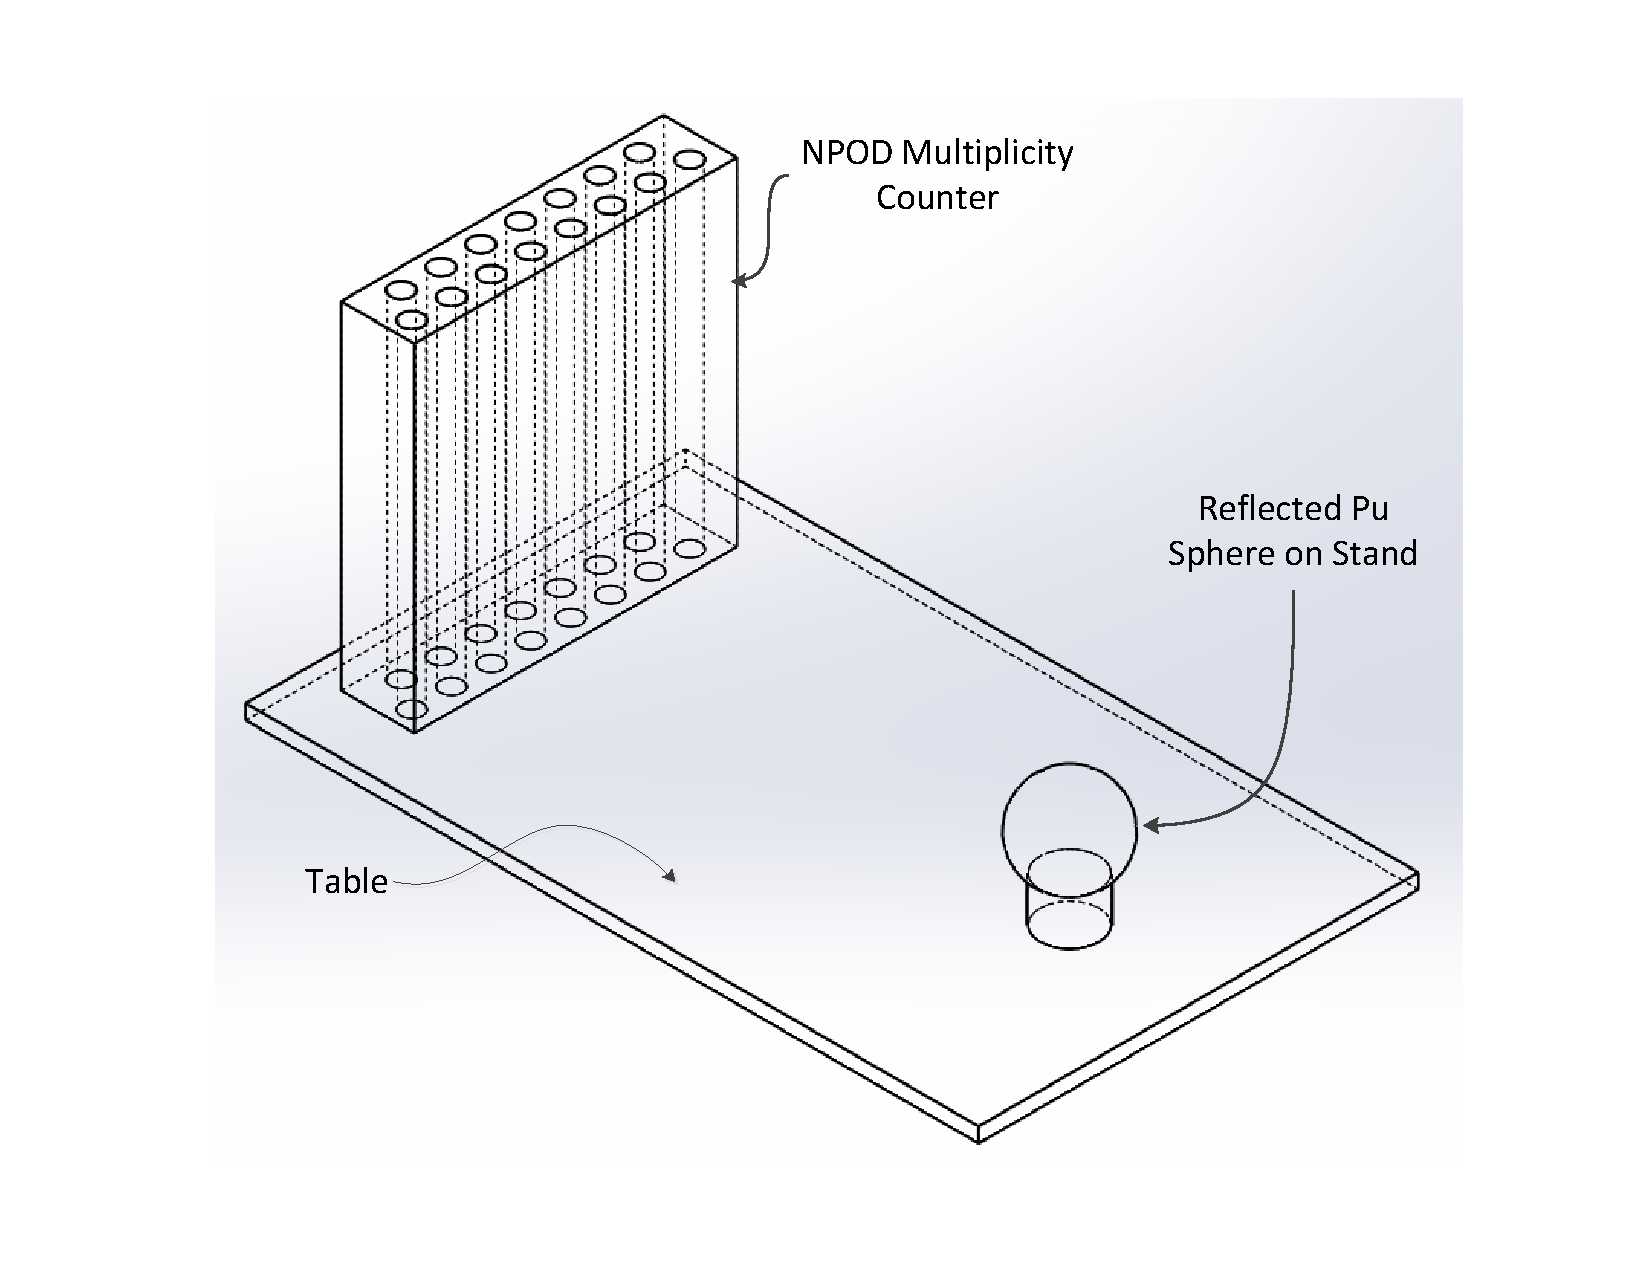
\includegraphics[trim=1.0in 0.70in 0.8in 0.50in,clip,width=1.19\textwidth]{multiplicity_experiment.pdf} \\
    {\fontsize{7pt}{6pt}\selectfont  *Not to scale}
\end{center}
\end{figure}
\end{minipage}
\begin{minipage}{0.54\linewidth}
    {\addtolength\leftmargini{-0.5in}
     \addtolength\leftmarginii{-0.2in}
     \addtolength\wideitemsep{0.1in}
\begin{itemize}
    \item[] Experimental Parameters
  \begin{itemize}
      \item 94\% \colb{\iso{Pu}{239}} sphere \vspace{-0.2in}
      \item 5 Different HDPE shells \\ \colG{From none to 3.0 cm HDPE}
  \end{itemize}
  \item[] Experiments repeated w/ \colb{\iso{Cf}{252}}
\end{itemize} 
}
\end{minipage}

\end{frame} 


\begin{frame}
    \frametitle{MCNP5 multiplicity simulations showed discrepancy \\ with experiments for
        Pu but not for \iso{Cf}{252}}
\begin{minipage}{0.41\textwidth}
\begin{figure}[ht!]
\begin{center}
	{
	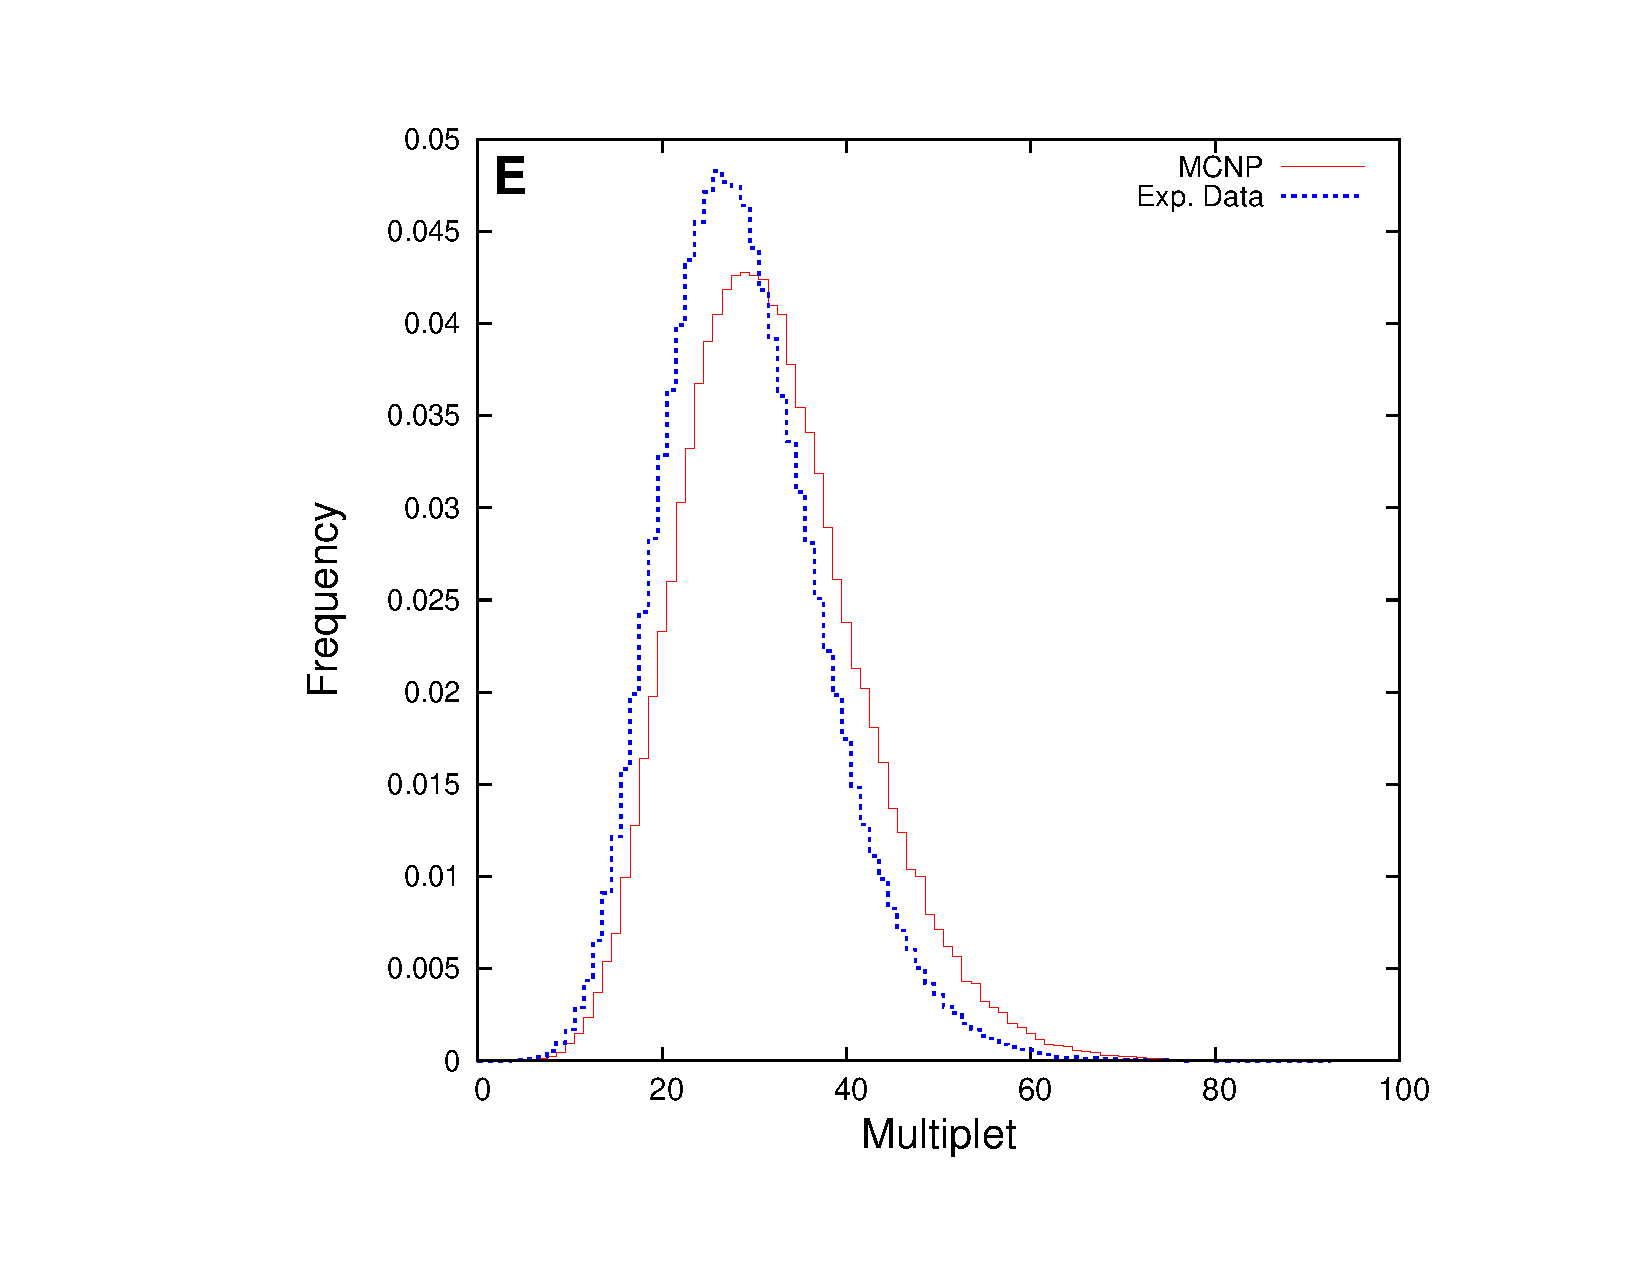
\includegraphics[trim= 2.00in 0.75in 1.450in 0.85in, clip, width=1.00\textwidth]{nubarFigures/trial_1_0_berp_3_0_2000.pdf} \\
	{\footnotesize Pu with 3.0-cm HDPE reflector} }
\end{center}
\end{figure} 
\begin{figure}[ht!]
\begin{center}
\end{center}
\end{figure} 

\end{minipage}
\begin{minipage}{0.56\textwidth}
    {\fontsize{10.8pt}{10pt}\selectfont
    \addtolength\leftmargini{-0.5in}
     \addtolength\leftmarginii{-0.2in}
     \addtolength\wideitemsep{0.1in}
\begin{itemize}
  \item[] Previous work by Mattingly [2010]
      \vspace{-0.1in}
  \begin{itemize}
      \item Caused by \textbf{\iso{Pu}{239}} \colb{nuclear data} 
	\vspace{-0.1505in}
	\item  Adjusted \colb{energy-integrated \nubar}	
	\end{itemize}
\item[]  In \textbf{ENDF-VII}, raised \nubar for \iso{Pu}{239} \\ \colG{to match \keff
    benchmarks}
    \vspace{0.1in}
  \begin{itemize}
 		\item \nubar is $\sim2\,\sigma$ \colr{above} measured data for $E < 1.5$ MeV 
	\end{itemize} 
\end{itemize} }
\end{minipage}
\end{frame} 
\begin{frame}
\frametitle{Can we reduce discrepancy in multiplicity distributions \\ without significantly
altering \keff?}
{\addtolength\leftmargini{-0.2in}
 \addtolength\wideitemsep{0.1in}
\begin{itemize}
    \item[] Perform energy-\colb{dependent} perturbations of $\overline{\nu}(E)$  in
        \iso{Pu}{239} \\ \colG{Random samples drawn from ENDF-VII.1 covariance data}
    \item[] Compare experimental and simulated multiplicity dist. 
            \\ \colG{and a $\keff$ benchmark (Jezebel)}
        \item[] Compare $\overline{\nu}(E)$ results to uniform shifts of
		microscopic cross sections 
	\end{itemize}	
}
\end{frame} 





%\section{Correlated Sampling}
%\subsection{Simulations of Multiplicity Experiments with Nuclear Data Perturbations}


%\section{Methodology}
%\subsection{Simulations of Multiplicity Experiments with Nuclear Data Perturbations}




\begin{frame}
\frametitle{We used LANL NDVV Python tools \\ to generate energy-dependent \nubar  samples}
{\addtolength\wideitemsep{0.2in}
\begin{enumerate}
	\item Generate a correlated sample of $\nubar(E)$ 
        \begin{itemize}\vspace{0.1in}
            \item {Assumed multivariate
                    Gaussian \\ \colG{ with group-averaged covariances}}
    \end{itemize}
  \item Modify continuous $\nubar(E)$ data in \textbf{ACE} file 
  \item Perform all MCNP simulations \\ \colG{with modified ACE data}
\end{enumerate} 
}
\end{frame} 



\begin{frame}
\frametitle{A cost function provides a measure \\ of inaccuracy for each data realization}
\begin{itemize}
	{
    \item[] \colb{Reduced} $\chi^2$ values for the 5 multiplicity experiments and criticality benchmark
        \begin{equation*} \hspace{0.4in}
		\begin{array}{c} 
            \displaystyle	\chi^2_{\text{red,mult,}m} = \frac{1}{N_{bins}-1}\sum_{i=1}^{N_{bins}}
	\frac{(P^{\textrm{exp}}_i - P^{\textrm{mcnp}}_i)^2}{\sigma^2(P^{\textrm{exp}}_i) + 
\sigma^2(P^{\textrm{mcnp}}_i)} 
		\end{array}
	\end{equation*} 
    \vspace{0.0in}
\item[] Equally weight $\chi^2$ values in a \colb{cost} function \\ \colG{A lower score indicatese
    higher accuracy}
	\begin{equation*}
        \boxed{\text{Cost} = \sum_{m=1}^5 \chi^2_{\text{red,mult,}m} + \chi^2_{\text{red,}\keff}}
	\end{equation*} 
}
\end{itemize}

\end{frame} 

%\begin{frame}
%\frametitle{Summary of Procedure}	
%\begin{itemize}
%	\item \colg{FOR} each \colb{trial} :
%	\begin{enumerate}
%		\item Generate a unique set of perturbed nuclear data
%		\item Run \textbf{MCNP5\_mult} simulations (5 multiplicity, \colb{JEZEBEL})
%		\item Produce multiplicity distributions
%		\item Compute $\chi^2_{red}$ values and cost
%	\end{enumerate} 
%	\item The \colb{lowest} cost is the most accurate trial
%\end{itemize}
%\end{frame} 


%\section{Results}
%\subsection{Simulations of Multiplicity Experiments with Nuclear Data Perturbations}

\begin{frame}
 \frametitle{Multiplicity and $\keff$ simulations were performed \\ for 500 unique realizations  of \nubar data}
\begin{center}
\resizebox{!}{0.5in}{
 \begin{tabular}{ccc}
	 \hline {Trial} & {Cost} & {$\chi^2_{\,{k}_{\mathrm{eff}}}$} 
\\ \hline
\nubar -1.14\%	&	164.24	&		33.66	\\	
\textbf{303}	&	\textbf{197.07}	&	\textbf{4.18}	\\	
%243	&	264.3	&	261.33	&	2.97	\\	
\colg{{55}}	&	267.9	&	\colg{0.01}	\\	
Original	&	426.86	&	0.27	\\	\hline
\end{tabular}
}
\end{center}
\begin{itemize}
    \item[]{MCNP criticality test suite performed for best data}
        \\ \colG{which includes 39 criticality benchmarks w/ \iso{Pu}{239}}:
\end{itemize}
	\begin{center}
\vspace{0.01in}
\resizebox{!}{0.50in}{
 \begin{tabular}{cc}
    \hline {Trial} & {$RMSD$} \\ \hline
\nubar -1.14\% & 1.23\% \\	
\colb{303} & \colb{0.51\%}	 \\
Original	&	0.49\% \\	\hline
\end{tabular}
}
\end{center}
\end{frame} 


\begin{frame}
\frametitle{Energy-dependent \nubar perturbations   \\ improved all 5 multiplicity
distributions}
\begin{itemize}
    \item Plots for best data realization and 3.0 cm HDPE case
\end{itemize}
\begin{center}
$\begin{array}{cc} \textbf{Original \nubar Data} & \hspace{0.13in}\textbf{Trial 303: Lowest Cost} \\
   \hspace{-0.25in}
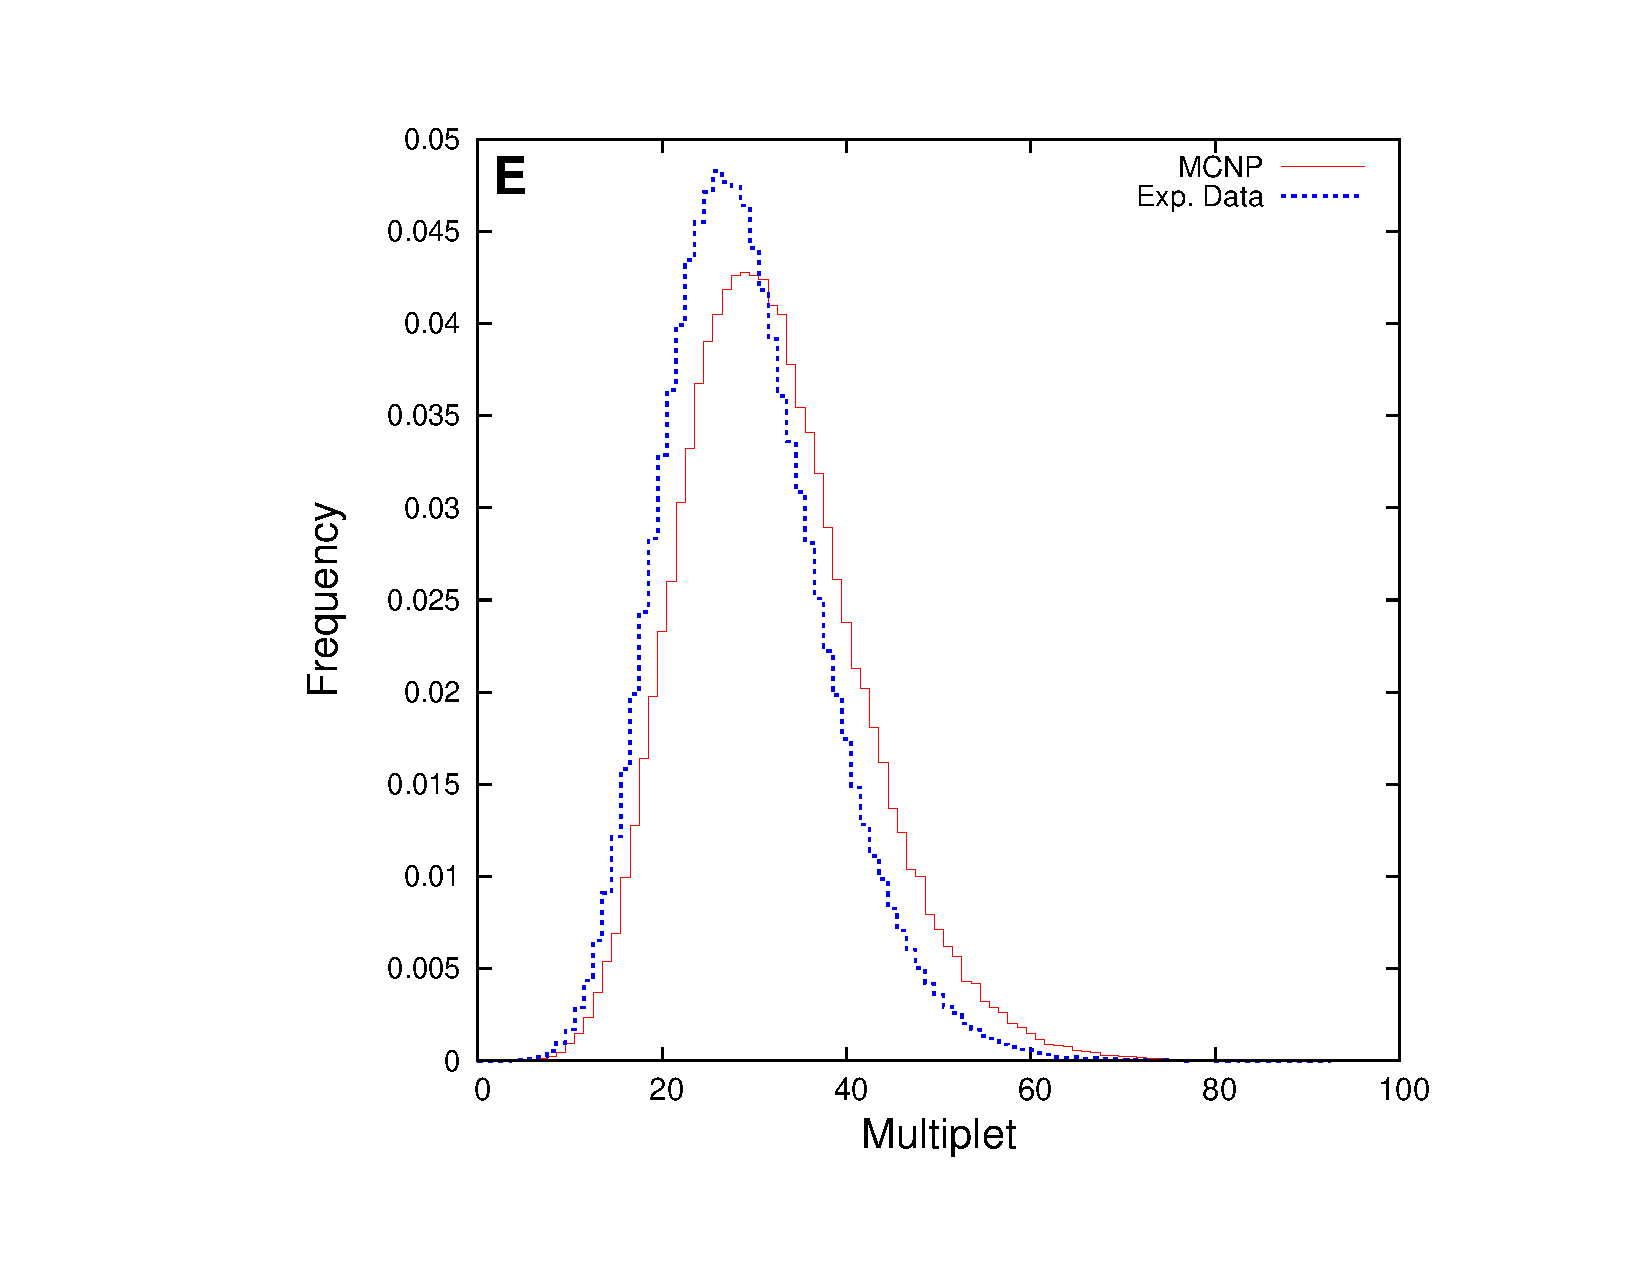
\includegraphics[trim= 1.0in 0.75in 1.0in 0.75in, clip, width=0.5\textwidth]{nubarFigures/trial_1_0_berp_3_0_2000.pdf} &
\hspace{-0.2in}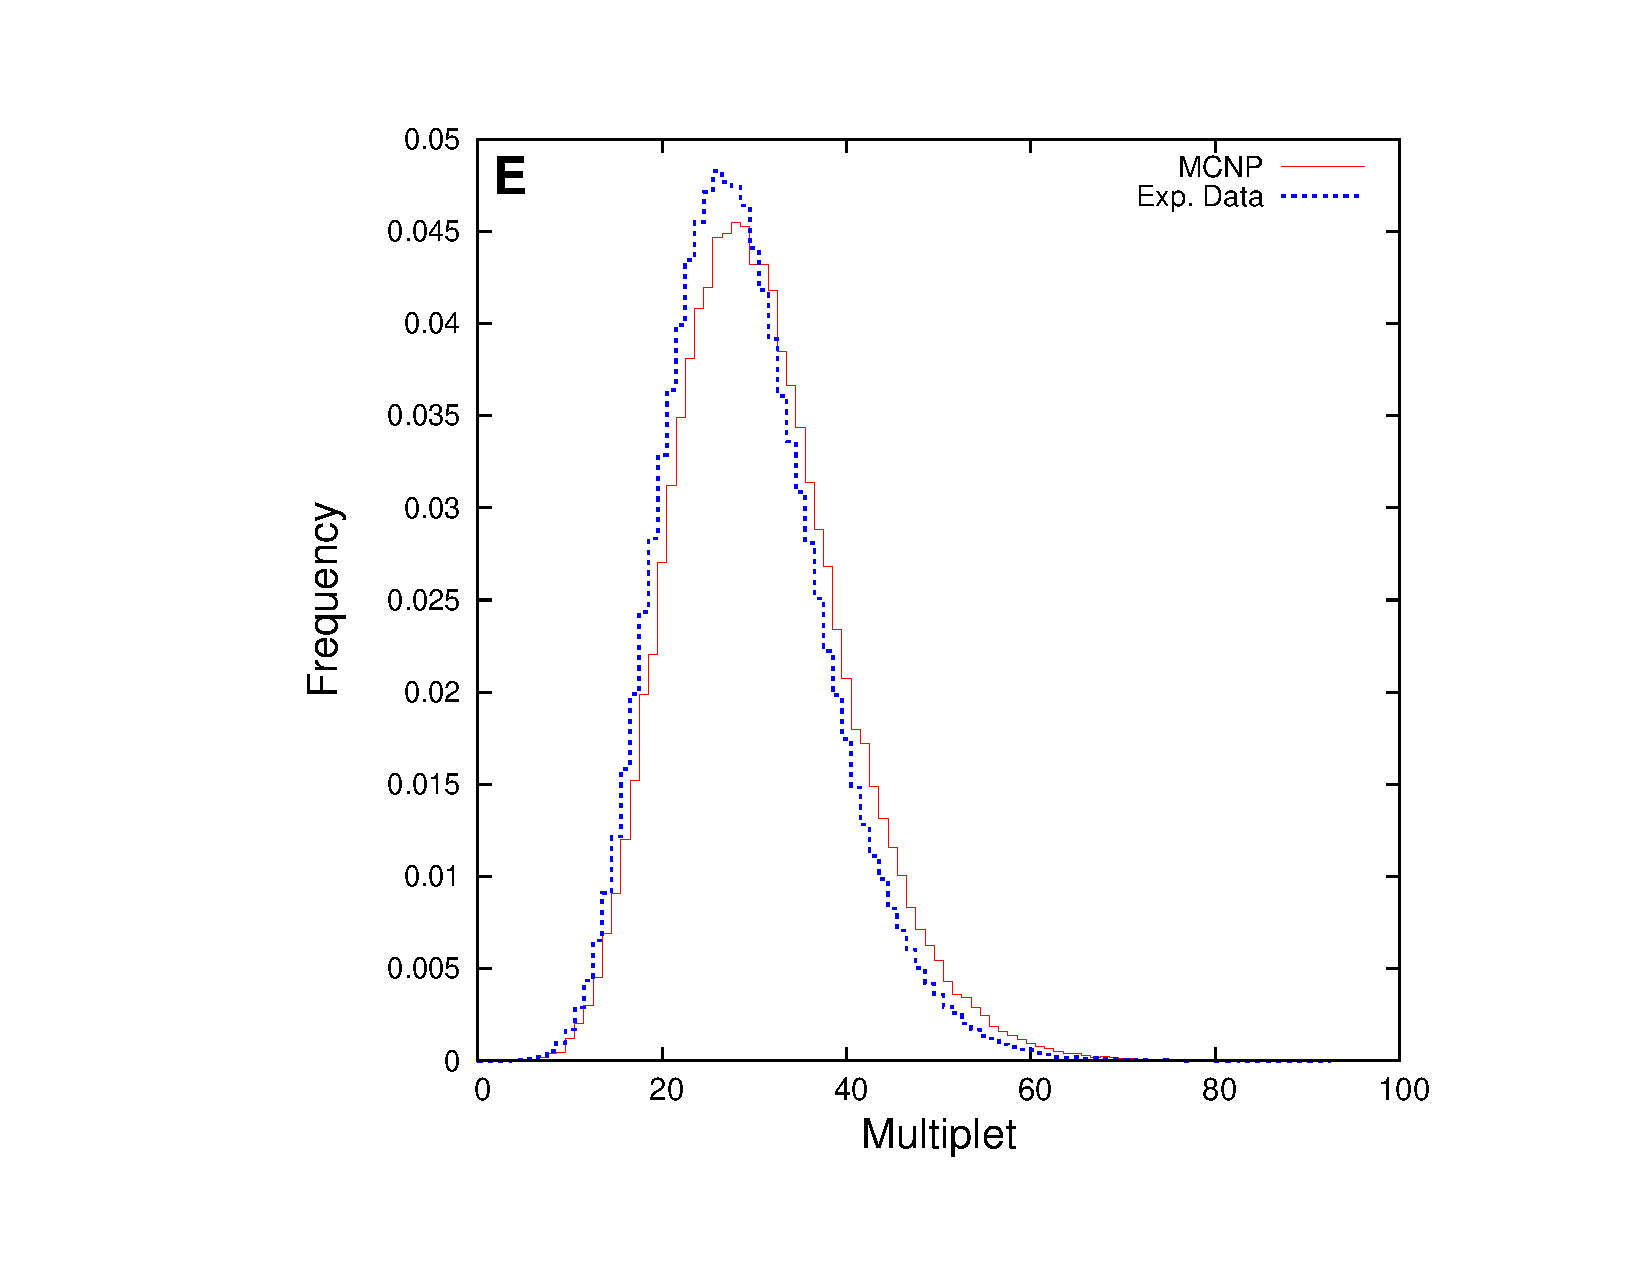
\includegraphics[trim=1.0in 0.75in  1.0in  0.75in, clip, width=0.5\textwidth]{nubarFigures/trial_303_berp_3_0_2000.pdf} \\
\end{array}$
\begin{itemize} 
	\item Best data set reduced \colb{bias} in {1$^{\text{st}}$} and {2$^{\text{nd}}$} moments, averaged over all 5 simulations, by \colb{$\sim35\%$}
\end{itemize}
\end{center}
\end{frame}


\logo{}

%\begin{frame}
%\frametitle{Capture Cross Section -- \coly{3.0 cm HDPE reflector}}
%{\small
%\begin{itemize} \vspace{-0.2in}
%	\item Adjust \colb{total cross section} ($\sigma_t$) to compensate for change in $\sigma_c$
%
%	\end{itemize} }
%	
%\begin{center}
%$\begin{array}{cc} \textbf{Original \sa Data} & \hspace{0.13in} {\sigma_c} \textbf{ increased 16\%} \\
%   \hspace{-0.25in}
%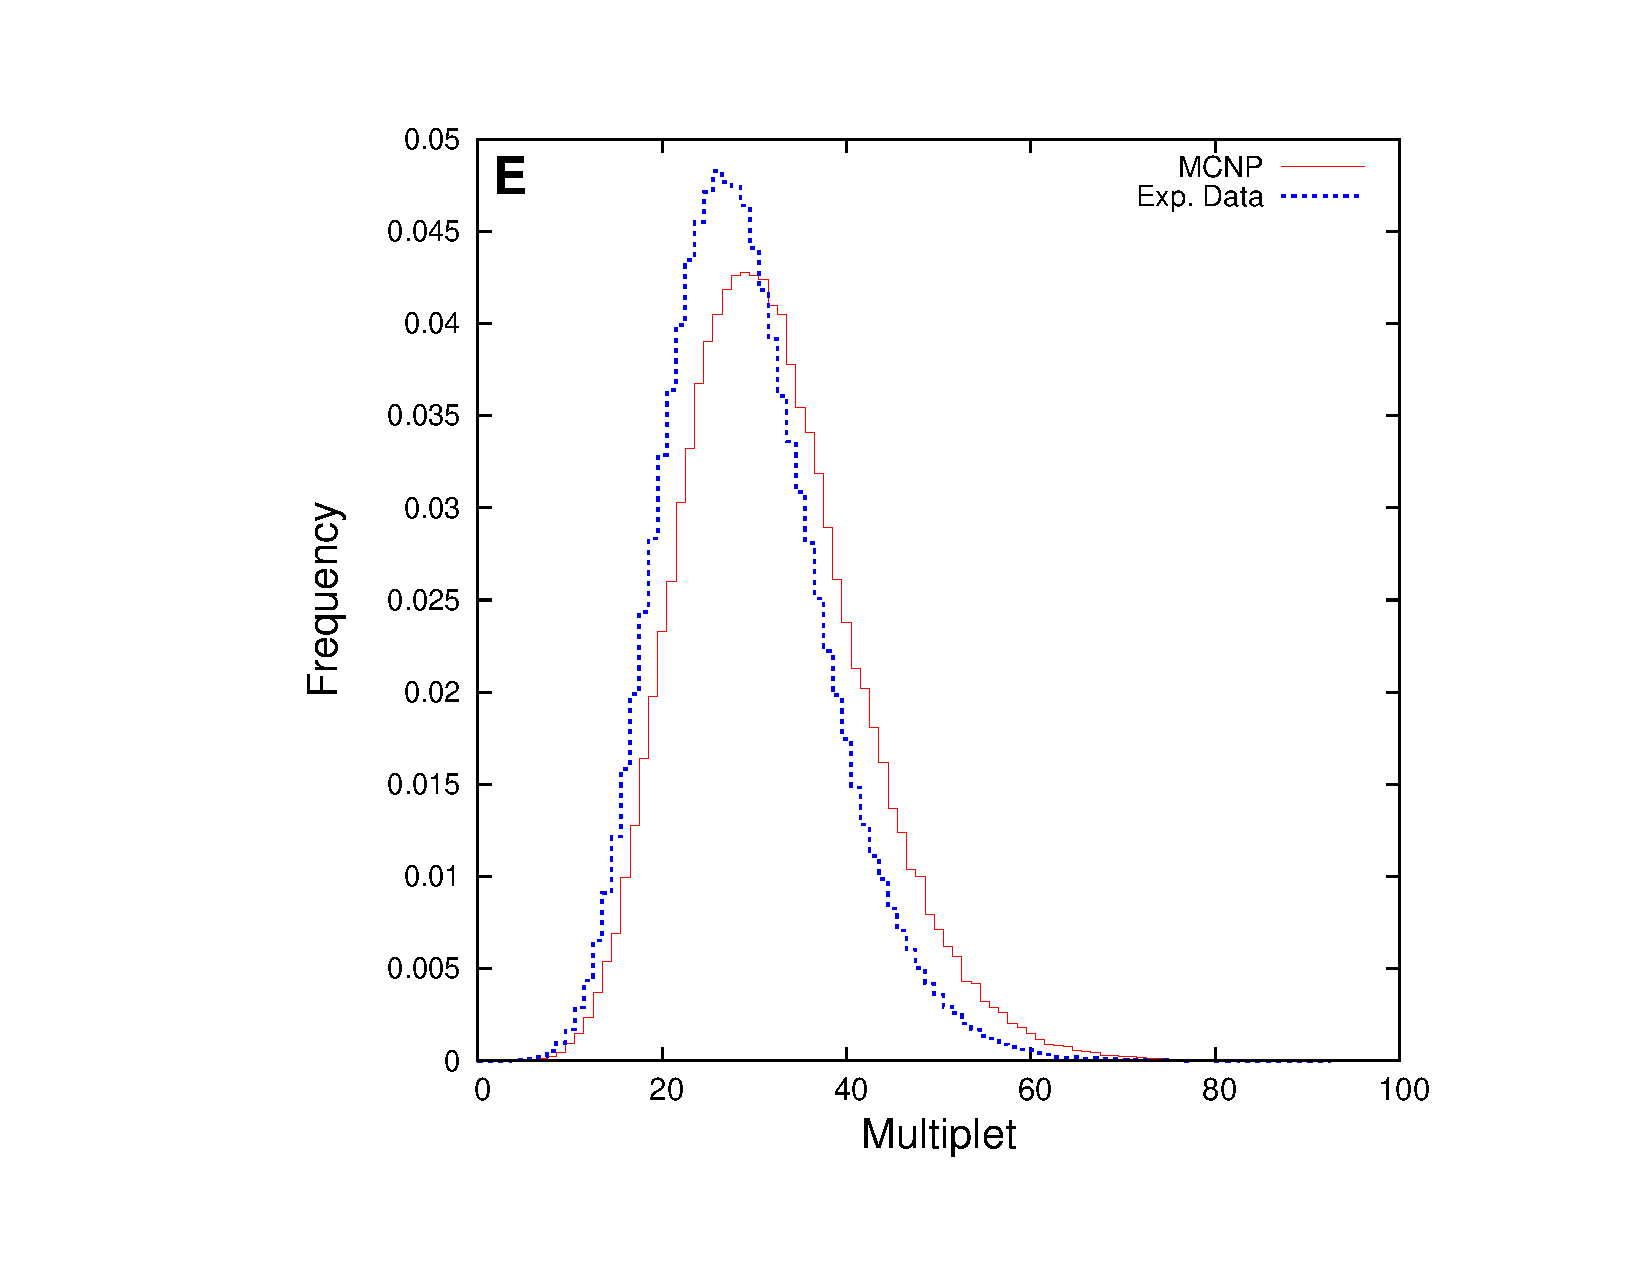
\includegraphics[trim= 1.0in 0.75in 1.0in 0.75in, clip, width=0.5\textwidth]{nubarFigures/trial_1_0_berp_3_0_2000.pdf} &
%\hspace{-0.2in}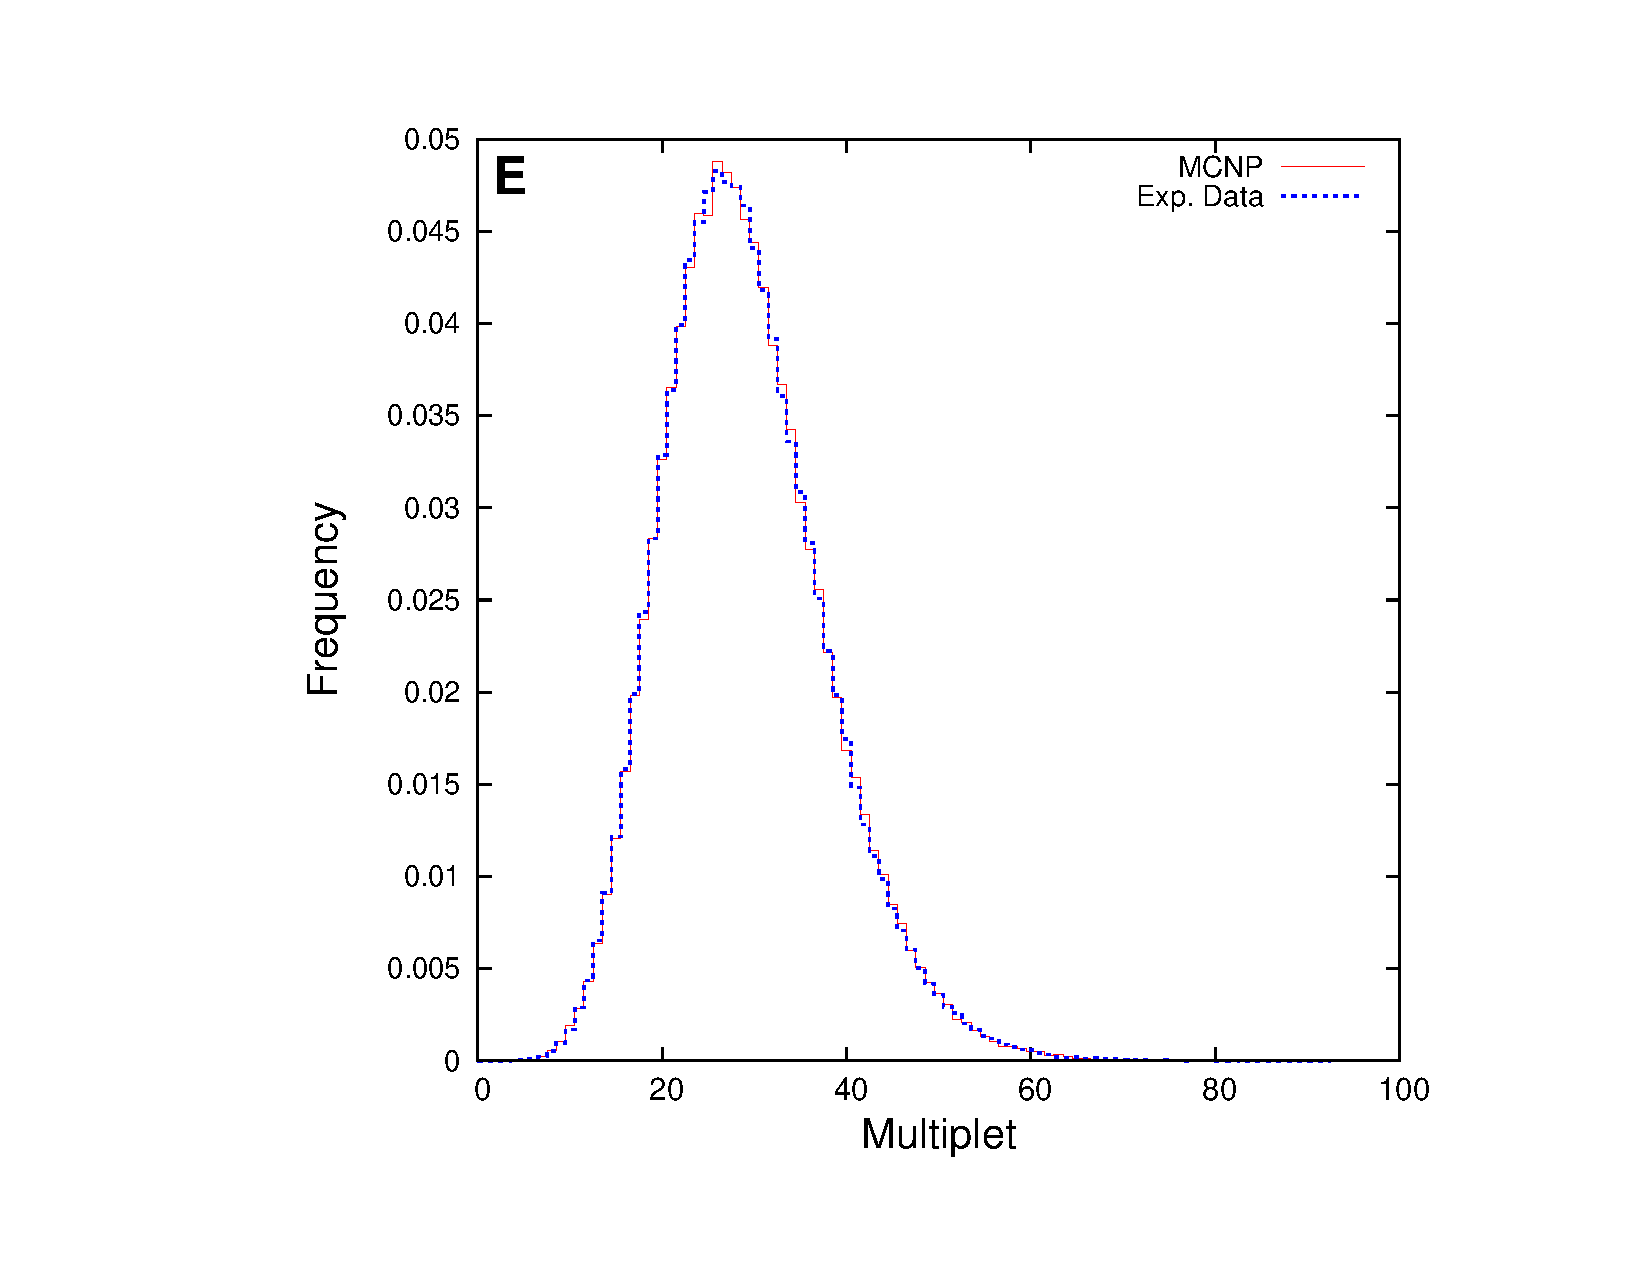
\includegraphics[trim=1.0in 0.75in  1.0in  0.75in, clip, width=0.5\textwidth]{capFigures/trial_16_0_berp_3_0_2000.pdf} \\
%\end{array}$
%\begin{itemize} 
%	\item Correction is \colr{less} for other experiments, and $\# s(\sigma_c) = \colr{7\;\sigma}$
%\end{itemize}
%\end{center}
%\end{frame}


\begin{frame}
    \frametitle{Adjusting the fission cross section \textbf{uniformly} \\ showed good correction to multiplicity
simulations}
\begin{center}
$\begin{array}{cc} \textbf{Original \sfiss Data} & \hspace{0.13in}\textbf{\sfiss decreased
    1.5\%} \\[6pt]
   \hspace{-0.25in}
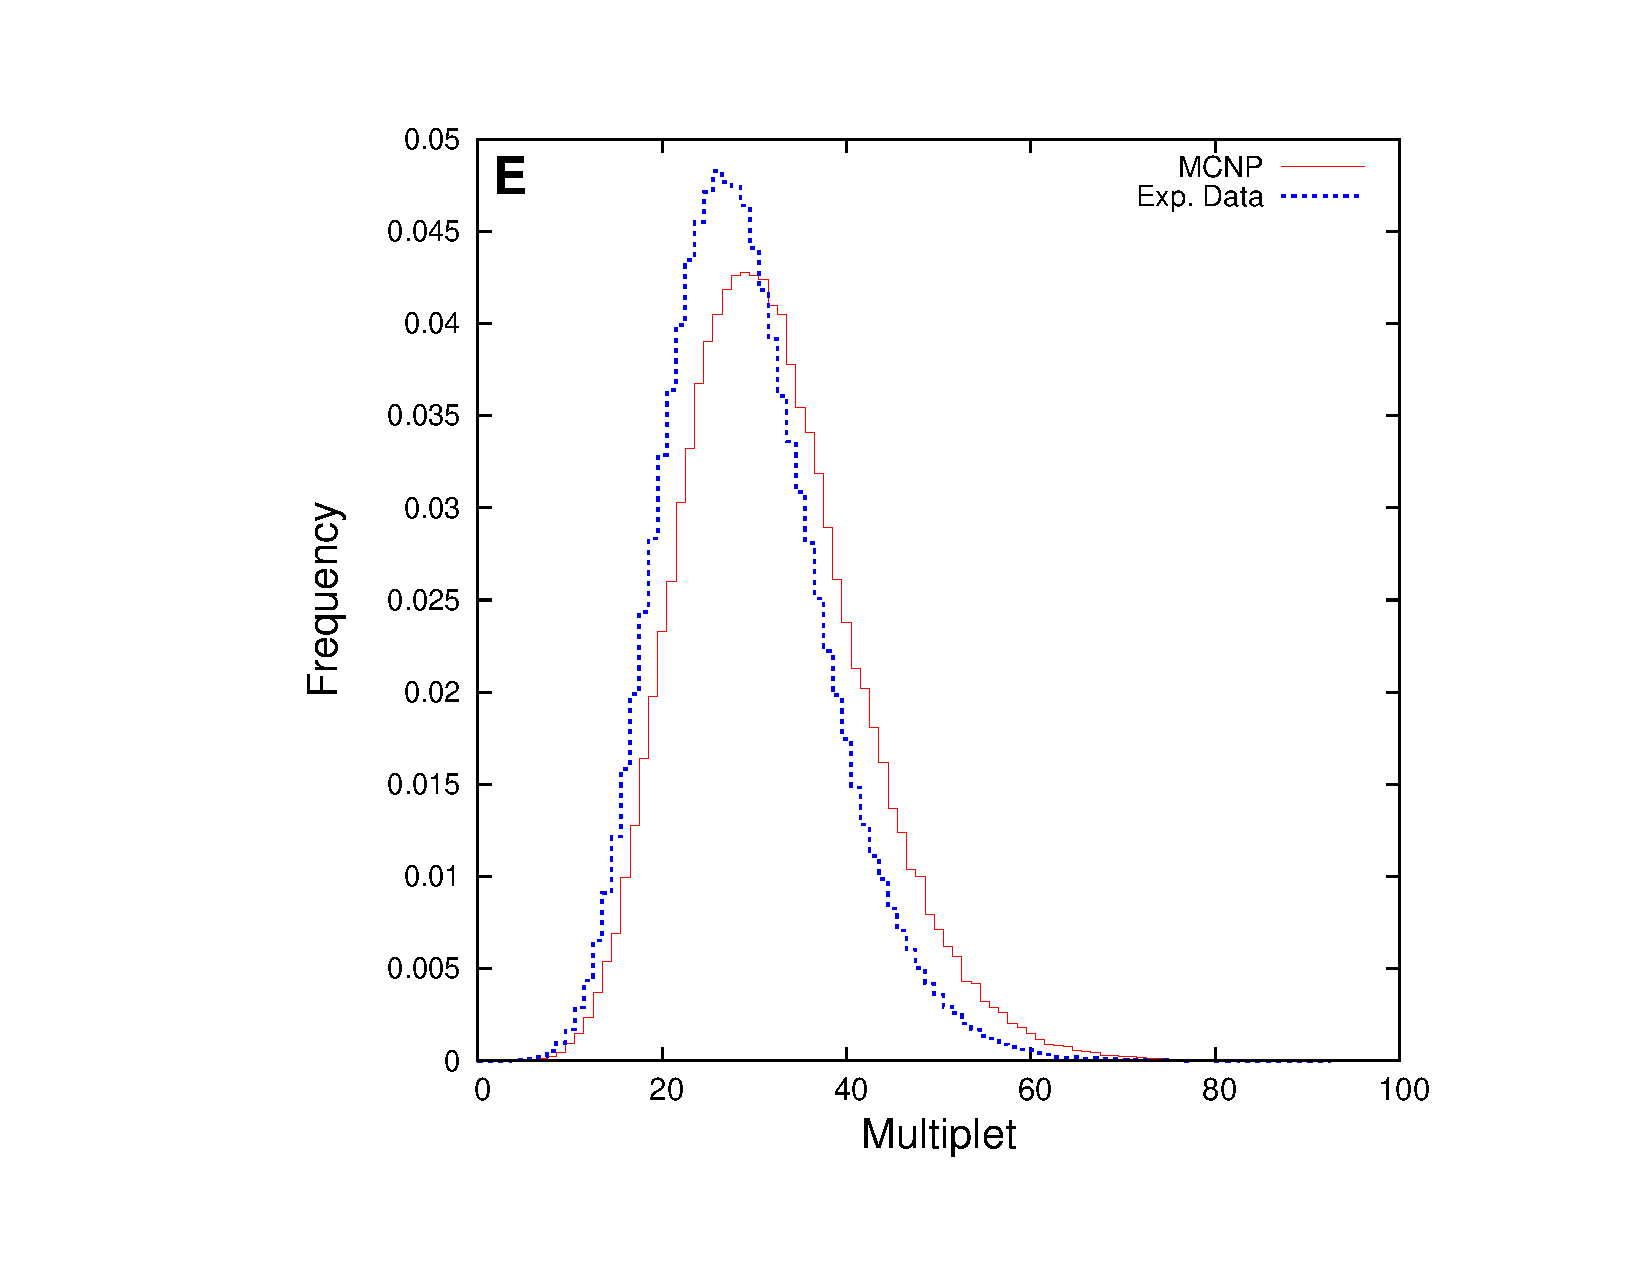
\includegraphics[trim= 1.0in 0.75in 1.0in 0.75in, clip, width=0.5\textwidth]{nubarFigures/trial_1_0_berp_3_0_2000.pdf} &
\hspace{-0.2in}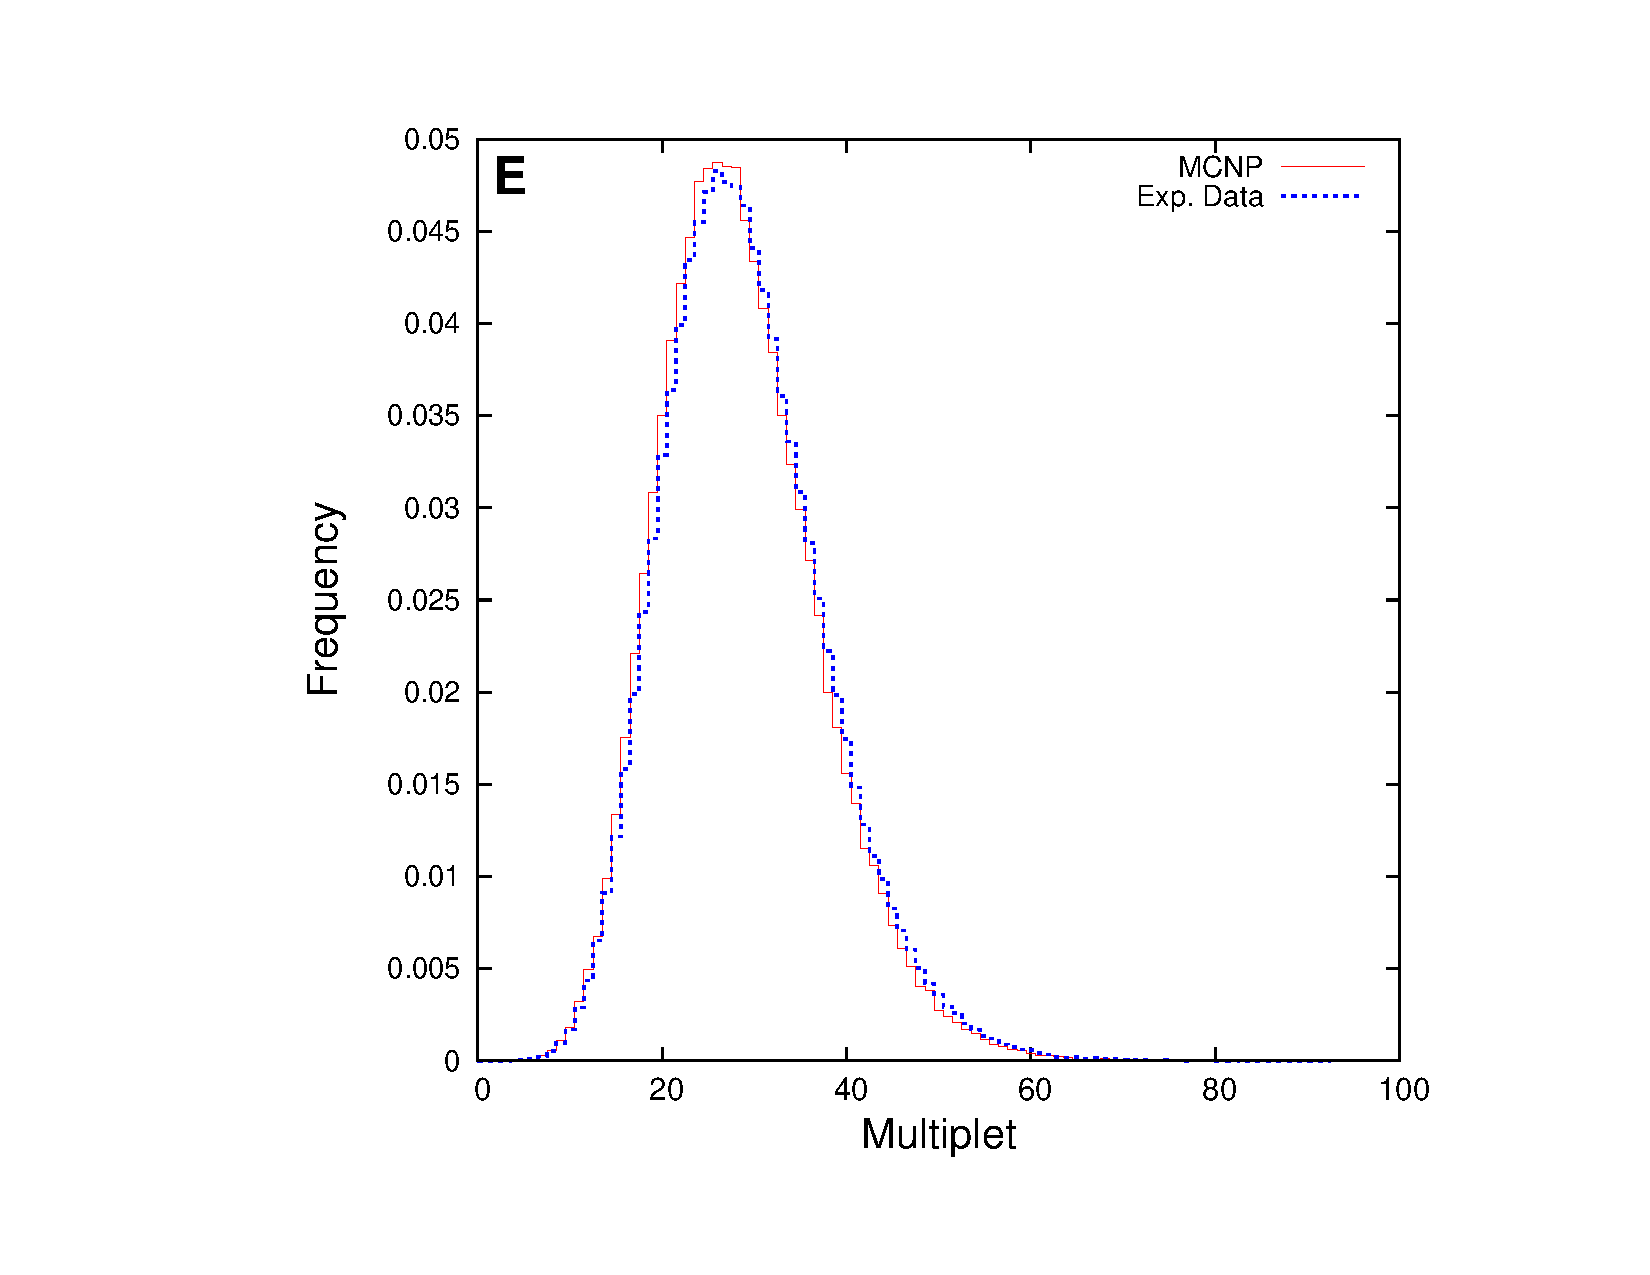
\includegraphics[trim=1.0in 0.75in  1.0in  0.75in, clip, width=0.5\textwidth]{capFigures/trial_-1_5_berp_3_0_2000.pdf} \\
\end{array}$
\end{center}
\begin{itemize} \vspace{-0.1in} 
  \item High accuracy for all simulations: $\displaystyle \sum_{i=1}^5 \chi^2_{red,mult,m} = \colb{14.6}$
      \vspace{-0.2in}
  \item \keff is \textbf{not preserved:} $\chi^2_{\keff} = 22.6$
\end{itemize} 
\end{frame}






%\section{Conclusions}
%\subsection{Simulations of Multiplicity Experiments with Nuclear Data Perturbations}
\begin{frame}
\frametitle{Simulations of Multiplicity Experiments \\ with Nuclear Data Perturbations}
	\vspace{-0.2in}
\begin{itemize}
    \item[] Energy-dependent \nubar perturbations \colb{reduced inaccuracies} in multiplicity while \colb{preserving} \keff
      \begin{itemize}\vspace{0.1in}
		\item Majority of cross-correlation terms $\mathcal{O}(10^{-4})$ or less
            \vspace{-0.1in}
        \item $\sigma_f$ may need more investigation
            \\ \colG{not sensitive to capture cross section}
	  \end{itemize}
      \item[] Subcritical simulations should be considered \\ in validation of nuclear data
      \item[] Covariance sampling methodology for nuclear data was developed and demonstrated
	\begin{itemize}
	 	\item Ideally sample all cross sections and \nubar simultaneously 

\end{itemize} 
\end{itemize}
\end{frame} 


\author{S.R. Bolding\inst{1}, \and C.J. Solomon\inst{2}}
\date{4 August 2016}
\begin{frame}
\vspace{-0.2in}
\centering
\maketitle

\end{frame} 



























\author{Simon R. Bolding}




% ---------------------------- BACKUP ---------------------


\appendix
%backupslides
\newcounter{finalframe}
\setcounter{finalframe}{\value{framenumber}}

\author{}
\date{}
\title{Backup Slides}

\maketitle

\author{Simon R. Bolding}


\begin{frame}
\frametitle{Summary of Procedure}	
\begin{itemize}
	\pause
	\item \colg{FOR} each \colb{"Trial"}:
	\begin{enumerate}
		\item Generate a new set of perturbed nuclear data
		\item Run \textbf{MCNP5\_mult} simulations (5 multiplicity, \colb{JEZEBEL})
		\item Produce multiplicity distributions
		\item Compute $\chi^2_{red}$ values and FOM
	\end{enumerate} \pause
	\item The \colb{lowest} FOM is the most ``accurate'' trial
\end{itemize}
\end{frame} 

\begin{frame}
\frametitle{Sample Statistics}
\begin{itemize}
  \setlength{\itemsep}{12pt}
	\item Consider independent random samples $\{x_i:\; i=1,2,\ldots,N\}$ of a variable $X$ with some
					PDF $f(x)$

	\item  {\color{blue} Statistics} are some $f(x_1,x_2,\ldots,x_N)$
	\begin{itemize}

	  \item {\color{blue} Sample} Mean: $\displaystyle \overline{x} = \frac{1}{N} \sum_{i=1}^N x_i$
    \vspace{-3pt}
	  \item {\color{blue} Sample} Variance: $\displaystyle s^2 = \frac{1}{N-1} \sum_{i=1}^N (x_i - \overline{x}) ^2$

	\end{itemize} 

	\item As $N\rightarrow \infty$, approach {\color{green} population} (true) mean and variance

\end{itemize}
\end{frame}

 
 



\begin{frame}
\frametitle{Energy-dependent \nubar perturbations}
\begin{center}
\textbf{Comparison of Moments}

\setlength{\tabcolsep}{6pt}
\begin{table}[ht]
\begin{center}
\resizebox{0.9\textwidth}{!}{
\begin{tabular}{|c|c|c|c|c|c|c|c|c|c|}
\hline \multirow{2}{*}{Reflector} & \multirow{2}{*}{Moment} & \multicolumn{3}{|c|}{ENDF/B-VII.1 \nubar} & \multicolumn{3}{|c|}{Trial 303 \nubar} & \multicolumn{2}{|c|}{Experimental} \\ \cline{3-10}
& & Value & $\sigma_{rel}$ & $\#$ $\sigma$ away & Value & $\sigma_{rel}$ & $\#$ $\sigma$ away  & Value & $\sigma_{rel}$ \\ \hline       
\multirow{2}{*}{None}   &1  &   1.76E+001   &   2.68E-003   &   14.11   &   1.74E+001   &   2.68E-003   &   10.13   &   1.69E+001   &   1.38E-003   \\  
&   2   &   3.31E+002   &   2.94E-003   &   24.43   &   3.24E+002   &   2.95E-003   &   17.59   &   3.08E+002   &   1.52E-003   \\  \hline
\multirow{2}{*}{0.5}    &1  &   2.40E+001   &   2.67E-003   &   16.72   &   2.37E+001   &   2.67E-003   &   11.75   &   2.29E+001   &   1.51E-003   \\  
&   2   &   6.13E+002   &   2.90E-003   &   29.51   &   5.97E+002   &   2.90E-003   &   20.84   &   5.61E+002   &   1.65E-003   \\  \hline
\multirow{2}{*}{1.0}    &1  &   3.17E+001   &   2.66E-003   &   23.52   &   3.11E+001   &   2.66E-003   &   16.67   &   2.97E+001   &   1.77E-003   \\  
&   2   &   1.07E+003   &   2.89E-003   &   41.52   &   1.03E+003   &   2.89E-003   &   29.59   &   9.38E+002   &   1.93E-003   \\  \hline
\multirow{2}{*}{1.5}    &1  &   3.80E+001   &   2.67E-003   &   28.61   &   3.70E+001   &   2.67E-003   &   19.27   &   3.51E+001   &   1.84E-003   \\
&   2   &   1.54E+003   &   2.92E-003   &   50.25   &   1.46E+003   &   2.91E-003   &   34.14   &   1.32E+003   &   2.01E-003   \\  \hline
\multirow{2}{*}{3.0}    &1  &   3.19E+001   &   2.70E-003   &   34.04   &   3.06E+001   &   2.70E-003   &   19.44   &   2.90E+001   &   1.75E-003   \\
&   2   &   1.11E+003   &   3.04E-003   &   58.05   &   1.02E+003   &   3.03E-003   &   33.72   &   9.17E+002   &   1.96E-003   \\  \hline
\end{tabular}
}
\end{center}
\end{table}


\end{center}
\end{frame}


\begin{frame}[fragile]
\frametitle{Nuclear Data Formats}
\begin{itemize}
  \item \textbf{ACE} format 
\end{itemize}
\hrule
\vspace{-0.1in}
{\tiny
\begin{verbatim}
94239.70c  236.998600 2.53010E-08   08/25/07
94-Pu-239 at 293.6K from endf/b-vii.0 njoy99.248                         mat9437
   808738    94239    72098       48       45       14        0        6
        0        0        0        0        0        0        0        0
        1   360491   371402   371450   371498   371546   371594   598924
   598970   658265   658310   733847   805945   805959   805973   806478
   806492   806492   806506   808735   371781   808738   715724   724200
   724211   724253   724259        0        0        0        0        0
   1.00000000000E-11   1.03125000000E-11   1.06250000000E-11   1.09375000000E-11
	\end{verbatim}}
\begin{itemize}
	\vspace{-0.05in}
	\item \textbf{ENDF} format
\end{itemize}
\hrule
\vspace{-0.1in}
{\tiny
	\begin{verbatim}
7.000000+6 4.519930-9 7.520000+6 0.000000+0                      943715102   56
0.000000+0 0.000000+0          0          0          0          0943715  099999
0.000000+0 0.000000+0          0          0          0          09437 0  0    0
9.423900+4 2.369986+2          0          0          0          1943731452    1
0.000000+0 0.000000+0          0        452          0          1943731452    2
0.000000+0 0.000000+0          1          5       1326         51943731452    3
1.000000-5 8.000000-3 1.000000+2 2.000000+2 3.000000+2 5.000000+2943731452    4
\end{verbatim}}


\end{frame} 



\begin{frame}
\frametitle{Capture Cross Section - Case 4}
\begin{itemize}
  \item Adjust \colb{elastic scattering} ($\sigma_s$) to compensate for change in $\sigma_c$
	\begin{equation*}
	\begin{array}{ccc}
%	\boxed{
	\boxed{\sigma'_s = \sigma_s - \epsilon_c}\hspace{0.4in} &  \epsilon_c = \alpha\,\sigma_c &\hspace{0.4in} \sigma'_c = \sigma_c + \epsilon_c%}
	\end{array}
	\end{equation*}
	\item \colb{Only} {for} $E>1 keV$
\end{itemize} 

\begin{table}[h!] 
	\vspace{-0.1in}
  \begin{center}
	\resizebox{0.45\textwidth}{!}{
  \begin{tabular}{|cccc|}
   \hline Trial & $\chi^2_{\,mult}$ &
    $\chi^2_{\,{k}_{eff}}$ &  $\#s(\sigma_c)$ 
    \\ \hline
\nubar -1.14\% & 130.58 & 33.7 &  n/a \\ 
$\alpha=10.0\%$ & 345.1 & 0.22 & 4.04 \\
$\alpha=4.0\%$ & 390.9 & 0.01  & 1.62 \\
$\alpha=1.0\%$ & 417.9 & 0.01 & 0.40 \\
Original & 426.6 & 0.27 & 0 \\  \hline
  \end{tabular}}
  \end{center}
\end{table}

\end{frame} 


\begin{frame}
\frametitle{Fission Cross Section -- Case 1}
\begin{table}[h!tb] 
\begin{center} \begin{tabular}{|ccccc|}
\hline {Trial} & {$\chi^2_{\,mult}$} & {$\chi^2_{\,{k}_{eff}}$} &
{$\#s(\sigma_t)$} & {$s(\#s(\sigma_t))$} \\ \hline -4.0\% & 1318.2 & 167.72 &
-1.16 & 0.82\\ -2.0\% & 101.0 & 48.31 & -0.58 & 0.41\\ -1.6\% & 27.1 & 22.97 &
-0.47 & 0.33\\ -1.4\% & 17.4 & 22.79 & -0.41 & 0.29\\ -1.2\% & 23.1 & 14.25 &
-0.35 & 0.25\\ -1.0\% & 47.7 & 9.37 & -0.29 & 0.21\\ -0.5\% & 178.7 & 1.33 &
-0.14 & 0.10\\ \nubar -1.14\% & 130.58 & 33.7 & n/a & n/a \\ Original & 426.6 &
0.27 & 0 & 0  \\  \hline \end{tabular} \end{center} \end{table}


\end{frame} 


\begin{frame}
\frametitle{Changing Fission and Capture Cross Sections}
\begin{itemize}
  \item Adjust \colb{fission} to compensate for change in \colb{capture}
	\begin{equation*}
	\begin{array}{ccc}
%	\boxed{
	\boxed{\sigma'_f = \sigma_f - \epsilon_c}\hspace{0.4in} &  \epsilon_c = {\colb{-}}\alpha\,\sigma_f &\hspace{0.4in} \boxed{\sigma'_c = \sigma_c + \epsilon_c}%}
	\end{array}
	\end{equation*}
\end{itemize} 

\begin{table}[h!] 
	\vspace{-0.1in}
  \begin{center}
	\resizebox{0.45\textwidth}{!}{
  \begin{tabular}{|ccc|}
    \hline {Trial} & {$\chi^2_{\,mult}$} &
      {$\#s(\sigma_c)$} \\ \hline
		$\alpha = 10\%$ & 90.66 & 4.31 \\
    $\alpha = 4$\%  & 222.47 & 1.72 \\ 
    $\alpha = 2\%$  & 314.82 & 0.86 \\ 
    \nubar -1.14\%  & 130.58 & n/a \\
    Original\%      & 426.6  & 0.0 \\  \hline
  \end{tabular}}
  \end{center}
\end{table}
\pause
\begin{itemize}
  \item $\mathbf{\sigma_f >> \sigma_c}$ 

\end{itemize} 
\end{frame} 



\begin{frame}
\frametitle{Effect of altering \st}
Monoenergetic neutrons, \colr{unit} atom density, \colb{two} reaction types: $\sigma_t = \sigma_a + \sigma_b$
{\small
\begin{itemize}
\item Perturb $\sigma_a$:    $\displaystyle \sigma_a' = \sigma_a+\epsilon_a,\quad \sigma_t' = \sigma_t+\epsilon_t \quad \sigma_b'=\sigma_b$
\item Interaction Probability:
\begin{equation*}
\begin{array}{rcl}
P(\mathrm{Interaction }\; i, x) & =   &  P(\mathrm{Interaction},x)*P(\mathrm{Interaction }\; i \mid \mathrm{Interaction}, x) \\
                                       &  =  &  \left[1 - e^{-\sigma_tx}\right]\frac{\sigma_i}{\sigma_t},
\end{array} 
\end{equation*}
\item Probability for $\sigma_b'$:
\begin{equation*}
P'(\mathrm{Interaction }\; b) = p'_b(x) = \left[1 - e^{-\sigma_t^{\,\prime}x}\right]\frac{\sigma_b}{\sigma_t^{\,\prime}}
\end{equation*} 
\end{itemize}}
\end{frame} 

\begin{frame}
\frametitle{Effect of altering \st}
{\small
\begin{itemize}
  \item Expand probability for $\sigma_b'$ with Taylor series: 
	\begin{equation*}
	p_b'(x) = \left[1 -(1 - \sigma_t^{\,\prime}x +\frac{ (\sigma_t^{\,\prime}x)^2}{2} + \mathcal{O}(\sigma_t^{\,\prime 3}x^3))   \right]\frac{\sigma_b}{\sigma_t^{\,\prime}}
	\end{equation*} 
	\begin{equation*}
	p_b'(x)= \sigma_b\,x - \frac{\sigma_t^{\,\prime}x^2 }{2}-\mathcal{O}(\sigma_t^{\,\prime 2}x^3)). 
	\end{equation*}
  \item Change in probability:
	\begin{equation*}
\Delta p_b(x) = p_b'(x) - p_b(x) = - \frac{(\sigma_t^{\,\prime} - \sigma_t) x^2}{2} + \mathcal{O}((\sigma_t^{\,\prime 2}-\sigma_t^2)x^3)
\end{equation*}
\begin{equation*}\boxed{
\Delta p_b(x) = - \frac{\epsilon_a x^2}{2} + \mathcal{O}((\sigma_t^{\,\prime 2}-\sigma_t^2)x^3)}
\end{equation*}

\end{itemize} }


\end{frame} 

\begin{frame}
\frametitle{Simulations}
\pause
\begin{itemize}
  \item Perform \textbf{MCNP5\_mult} simulations
	\begin{itemize}
	\item Use modified nuclear data from created \textbf{ACE} files
  \item The 5 different Pu sphere \colb{multiplicity} experiments
	\item \colb{JEZEBEL} fast critical benchmark
	\end{itemize}
	\pause
	\item Generate multiplicity distributions with \textbf{mtool.pl} script
	\begin{itemize}
	  \item \colb{Non-paralyzable} dead time correction
	\end{itemize} 

\end{itemize}

\end{frame} 



\begin{frame}
\frametitle{Comparing Results of Simulations}
\begin{itemize}
	{\small \pause
	\item \colb{Reduced} $\chi^2$ values for the 5 multiplicity experiments and criticality benchmark
	\begin{equation*}
		\begin{array}{c} 
	\displaystyle	\chi^2_{red,mult,m} = \frac{1}{N_{bins}-1}\sum_{i=1}^{N_{bins}} \frac{(R_i - S_i)^2}{\sigma^2(R_i) + 
			\sigma^2(S_i)} 
		\\[5pt] \displaystyle \chi^2_{red,\keff} = \frac{(\keff^{\textrm{MCNP}} - \keff^{ref})^2}{\sigma^2(\keff^{\textrm{MCNP}}) + \sigma^2(\keff^{ref})}
		\end{array}
	\end{equation*} \pause
	\item Compute a \colb{FOM}:
	\begin{equation*}
	 \boxed{FOM = \sum_{m=1}^5 \chi^2_{red,mult,m} + \chi^2_{red,\keff}}
	\end{equation*} 
}
\end{itemize}

\end{frame} 

\begin{frame}
\frametitle{Modifying Nuclear Data}
\pause
\begin{itemize}
	\item<2-> Covariance data: \textbf{ENDF/B-VII.1} library
	\begin{itemize}
			\item<3-> \colb{Python} modules at LANL allow reading of ENDF files
			\item<4-> Integrated ability to handle \emph{certain} covariance data
			   \begin{itemize}
				\setlength{\itemsep}{0in}
			     \item<5-> Parsing data
				\vspace{-0.08in}
			    	\item<6-> Constructing full matrices
				\vspace{-0.08in}
				\item<7-> Sampling routines
			\end{itemize}
	\end{itemize} 
 	\item<2-> MCNP input nuclear data: \textbf{ACE} format
	\begin{itemize}
  	\item<8-> Built Python modules to read, modify, and rewrite nuclear data
	\end{itemize}
	\item<9-> Random samples of $\overline{\nu}(E)$, rather than \colb{linear optimization} (LO)
	\begin{itemize}
		\item<10-> LO would not preserve statistical accuracy
	  \item<10-> Under-constrained problem, \colb{infinite solutions}
\end{itemize} 
\end{itemize} 
\end{frame}

\begin{frame}
\frametitle{Capture Cross Section}	
\begin{itemize} 
	\item Adjust \colb{total cross section} ($\sigma_t$) to compensate for change in $\sigma_c$
	\begin{equation*}
	\begin{array}{ccc}
%	\boxed{
	\boxed{\sigma'_t = \sigma_t + \epsilon_c}\hspace{0.4in} &  \epsilon_c = \alpha\,\sigma_c &\hspace{0.4in} \sigma'_c = \sigma_c + \epsilon_c%}
	\end{array}
	\end{equation*}
	\end{itemize}
	\pause
\begin{minipage}{0.49\textwidth}
\begin{table}[t!] 
	\vspace{-0.63870in} \pause
  \begin{center}
	\resizebox{0.99\textwidth}{!}{
  \begin{tabular}{|ccccc|}
    \hline Trial & {$\chi^2_{\,mult}$} &
    {$\chi^2_{\,{k}_{eff}}$} &  {$\#s(\sigma_t)$}
  &   {$\#s(\sigma_c)$} 
   \\  \hline
    \nubar -1.14\% & 130.6 & 33.66 & n/a  & n/a \\
\colg{$\mathbf{\alpha=16.0\%}$} & \colg{142.6} & \colg{1.86} & \colg{3.47} & \colg{6.90}\\
$\alpha=8.0\%$ & 237.5 & 0.51 & 1.74 &  3.45 \\ 
$\alpha=2.0\%$ & 371.2 & 0.02 & 0.43 &  0.86 \\
$\alpha=1.0\%$ & 396.4 & 0.16 & 0.22 &  0.43 \\
Original & 426.6 & 0.27 & 0 & 0  \\ \hline
  \end{tabular}}
  \end{center}
\end{table}
\end{minipage}
\begin{minipage}{0.49\textwidth}
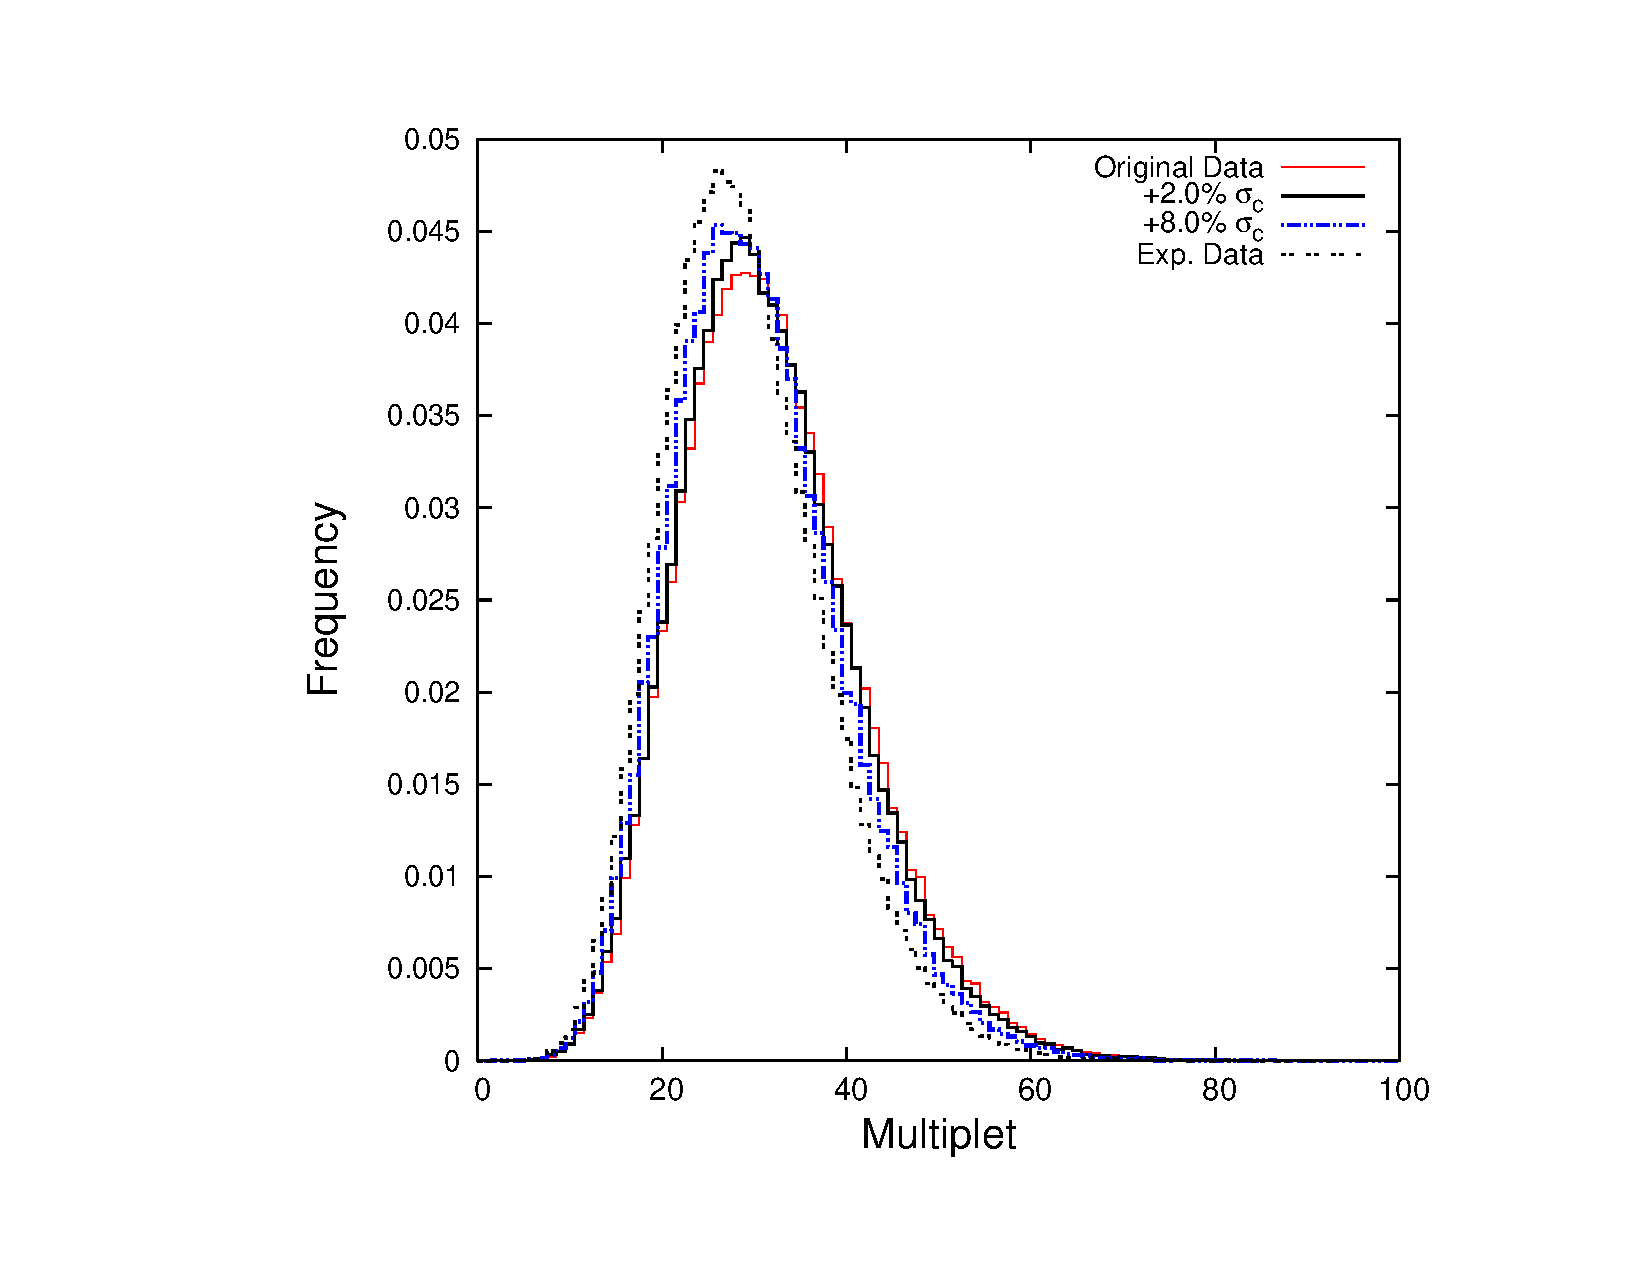
\includegraphics[trim=1.05in 0.75in 0.75in 0.75in, clip, width=1.099\textwidth]{capFigures/capture_3.pdf}
\end{minipage}	

\end{frame} 

\begin{frame}
\frametitle{Capture Cross Section}	
\begin{itemize} 
	\item Adjust \colb{total cross section} ($\sigma_t$) to compensate for change in $\sigma_c$
	\begin{equation*}
	\begin{array}{ccc}
%	\boxed{
	\boxed{\sigma'_t = \sigma_t + \epsilon_c}\hspace{0.4in} &  \epsilon_c = \alpha\,\sigma_c &\hspace{0.4in} \sigma'_c = \sigma_c + \epsilon_c%}
	\end{array}
	\end{equation*}
	\end{itemize}
	\pause
\begin{minipage}{0.49\textwidth}
\begin{table}[t!] 
	\vspace{-0.63870in} \pause
  \begin{center}
	\resizebox{0.99\textwidth}{!}{
  \begin{tabular}{|ccccc|}
    \hline Trial & {$\chi^2_{\,mult}$} &
    {$\chi^2_{\,{k}_{eff}}$} &  {$\#s(\sigma_t)$}
  &   {$\#s(\sigma_c)$} 
   \\  \hline
    \nubar -1.14\% & 130.6 & 33.66 & n/a  & n/a \\
\colg{$\mathbf{\alpha=16.0\%}$} & \colg{142.6} & \colg{1.86} & \colg{3.47} & \colg{6.90}\\
$\alpha=8.0\%$ & 237.5 & 0.51 & 1.74 &  3.45 \\ 
$\alpha=2.0\%$ & 371.2 & 0.02 & 0.43 &  0.86 \\
$\alpha=1.0\%$ & 396.4 & 0.16 & 0.22 &  0.43 \\
Original & 426.6 & 0.27 & 0 & 0  \\ \hline
  \end{tabular}}
  \end{center}
\end{table}
\end{minipage}
\begin{minipage}{0.49\textwidth}
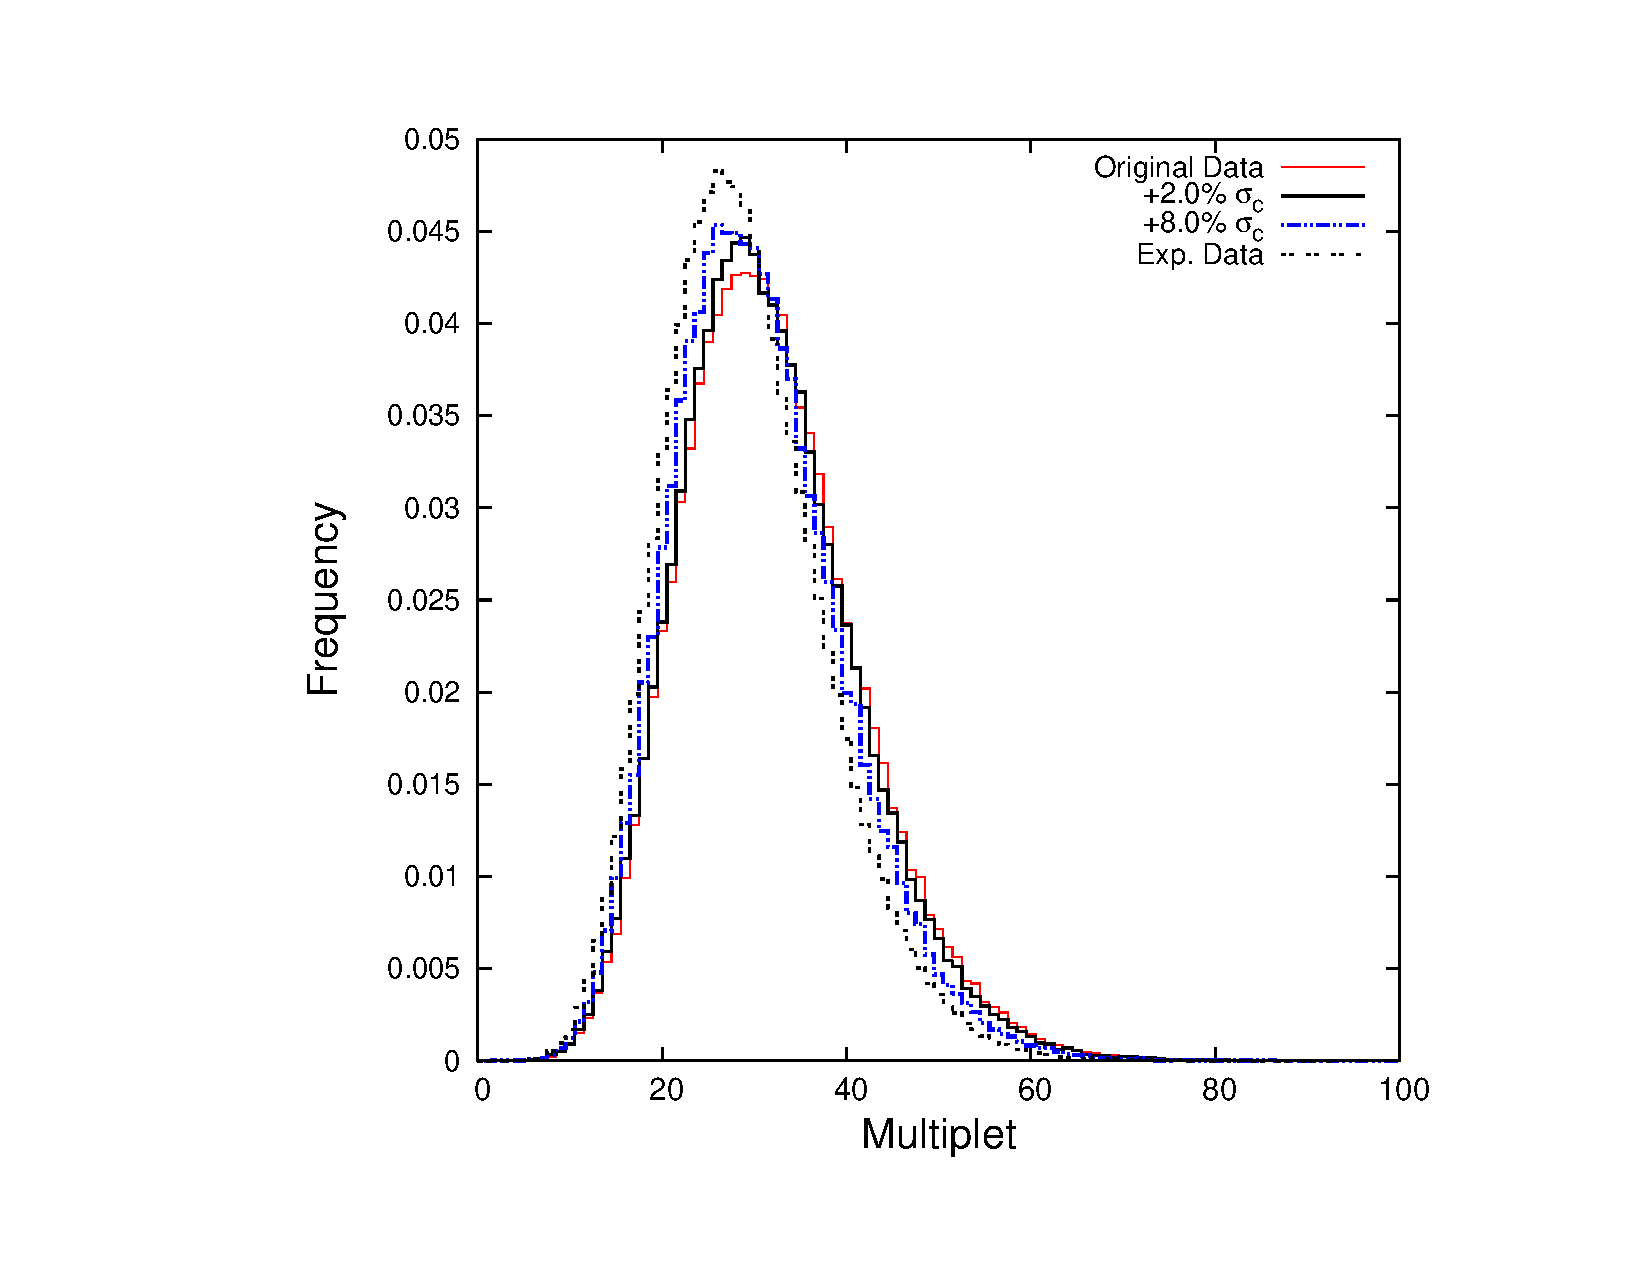
\includegraphics[trim=1.05in 0.75in 0.75in 0.75in, clip, width=1.099\textwidth]{capFigures/capture_3.pdf}
\end{minipage}	

\end{frame} 



\begin{frame}
\frametitle{Fission Cross Section}
\begin{itemize}
  \item Adjust \colb{elastic scattering} ($\sigma_s$) to compensate for change in $\sigma_f$
	\begin{equation*}
	\begin{array}{ccc}
%	\boxed{
	\boxed{\sigma'_s = \sigma_s + \epsilon_f}\hspace{0.4in} &  \epsilon_f = {\colb{-}}\alpha\,\sigma_f &\hspace{0.4in} \sigma'_f = \sigma_f \colb{-} \epsilon_f%}
	\end{array}
	\end{equation*}
	\item \colb{Only} {for} $E>1 keV$
\end{itemize} 
\pause

\begin{table}[h!] 
	\vspace{-0.1in}
  \begin{center}
	\resizebox{0.345\textwidth}{!}{
  \begin{tabular}{|ccc|}
    \hline {Trial} & {$\chi^2_{\,mult}$} &
    {$\chi^2_{\,{k}_{eff}}$}  \\ \hline
    $\alpha = 2.0$\% & 65.8 & 29.6 \\ 
    $\alpha = 1.5\%$ & 14.6 & 24.4 \\ 
    $\alpha = 1.0\%$ & 56.5 & 9.4 \\ 
    $\alpha = 0.5\%$ & 195.7 & 3.0 \\ 
   \nubar -1.14\% & 130.58 & 33.7 \\
    Original\% & 426.6 & 0.0  \\  \hline
  \end{tabular}}
  \end{center}
\end{table}

\end{frame} 

\begin{frame}
\frametitle{Future Work}
\vspace{-0.86in}
\begin{itemize}
  \item More energy-dependent \nubar trials \pause
%	\item Need covariance data for \sfiss and $\sigma_s$ \pause
	\item Energy-dependent \sfiss trials \pause
	\begin{itemize}
		\item \sfiss has \colb{400} covariance energy groups vs \colb{50} for \nubar
		\item Need constrained global optimization method
	\end{itemize}\pause



\end{itemize} 

\end{frame} 



\setcounter{framenumber}{\value{finalframe}}



\end{document}
